% article example for classicthesis.sty
\documentclass[10pt,a4paper]{article} % KOMA-Script article scrartcl
\usepackage{import}
\usepackage{xifthen}
\usepackage{pdfpages}
\usepackage{transparent}
\newcommand{\incfig}[1]{%
    \def\svgwidth{\columnwidth}
    \import{./figures/}{#1.pdf_tex}
}
\usepackage{lipsum}     %lorem ipsum text
\usepackage{titlesec}   %Section settings
\usepackage{titling}    %Title settings
\usepackage[margin=10em]{geometry}  %Adjusting margins
\usepackage{setspace}
\usepackage{listings}
\usepackage{amsmath}    %Display equations options
\usepackage{amssymb}    %More symbols
\usepackage{xcolor}     %Color settings
\usepackage{pagecolor}
\usepackage{mdframed}
\usepackage[spanish]{babel}
\usepackage[utf8]{inputenc}
\usepackage{longtable}
\usepackage{multicol}
\usepackage{graphicx}
\graphicspath{ {./Images/} }
\setlength{\columnsep}{1cm}

% ====| color de la pagina y del fondo |==== %
\pagecolor{white}
\color{black}



\begin{document}
    %========================{TITLE}====================%
    \title{\rmfamily\normalfont\spacedallcaps{ 4th Lab: Disassembly And IDAPro }}
    \author{\spacedlowsmallcaps{Rodrigo Castillo featuring Juen Esteban Murcia}}
    \date{\today}

    \maketitle


    %=======================NOTES GOES HERE===================%
    \section{Process monitor:}
        Here, my team started to capture events :
        \\
        \begin{figure}[h]
            \centering
            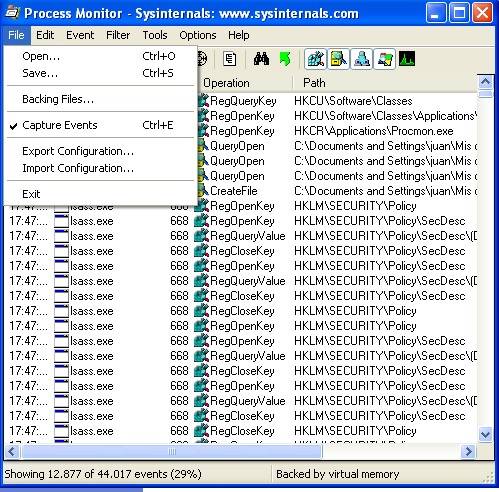
\includegraphics[width=0.4\linewidth]{capturandoeventos.jpeg}
            \caption{Event Capture}
            \label{1}
        \end{figure}
        \\
        then, we stop capturing events. :
        \begin{figure}[h]
            \centering
            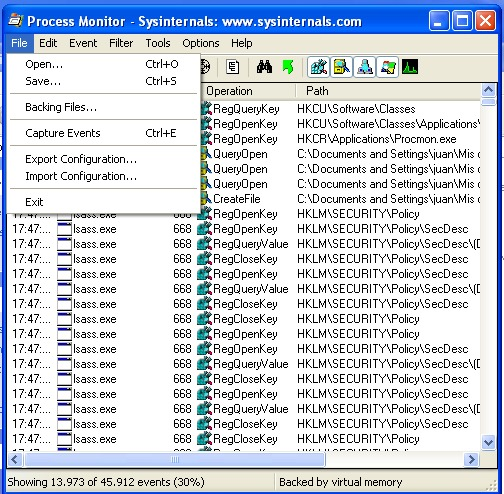
\includegraphics[width=0.4\linewidth]{fig2.jpeg}
            \caption{Stop Capturing events}
            \label{2}
        \end{figure}
        \newpage
        then, my team proceed to clean the dispay :
        \\
        \begin{figure}[h!]
            \centering
            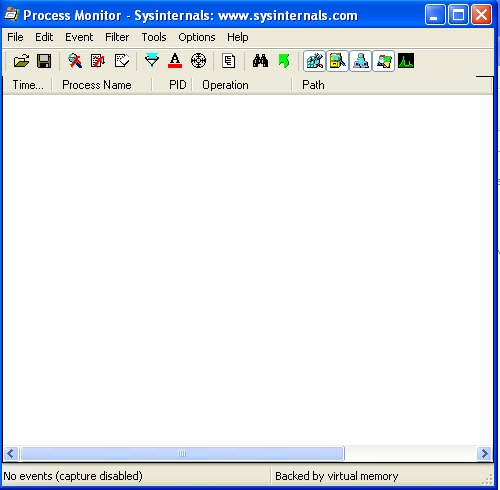
\includegraphics[width=0.4\linewidth]{fig3.jpeg}
            \caption{Cleaning Display}
            \label{3}
        \end{figure}
        \\ after this, my teem proceed to take the snapchot of  the machine
        before infecting it :
        \\
        \begin{figure}[h]
            \centering
            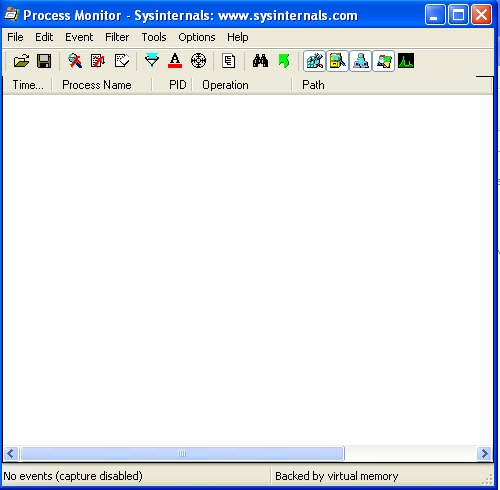
\includegraphics[width=0.4\linewidth]{fig3}
            \caption{Snapchot of the machine before running the malware}
            \label{4}
        \end{figure}
        \newpage
        At this point, we are able to review the events that redbear is
        running :
        \\
        \begin{figure}[h!]
            \centering
            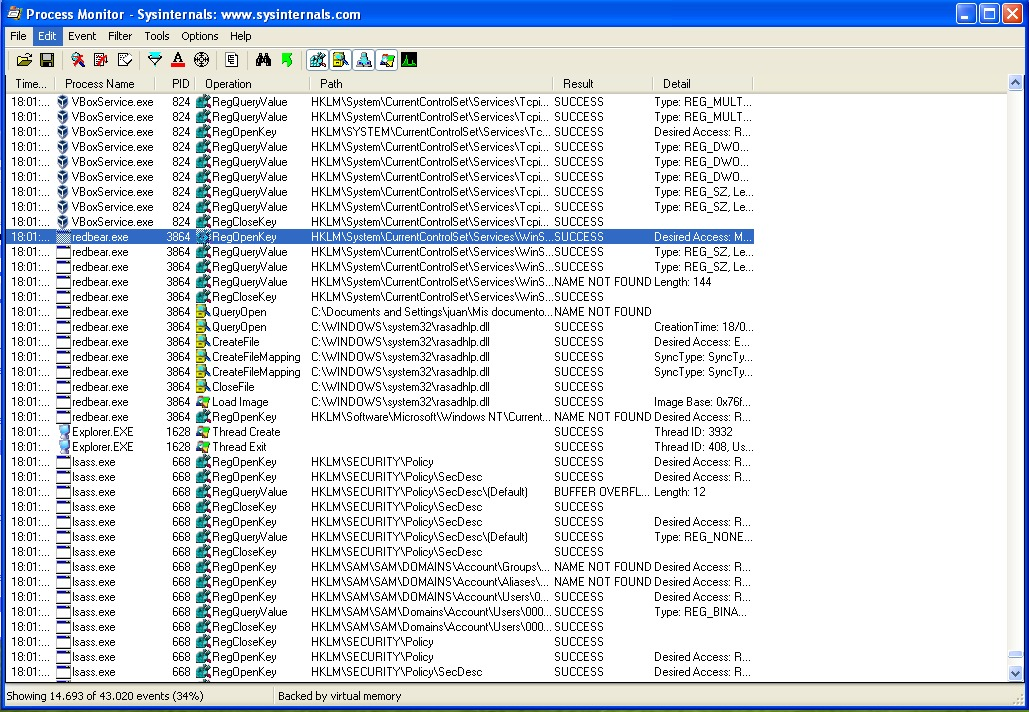
\includegraphics[width=0.8\linewidth]{fig5}
            \caption{Events that Redbear is running}
            \label{5}
        \end{figure}

        \\
        We can apreciete the keys and memory spaces where redbear is taking
        access , also, the .dll files he's calling and the files he is
        creating. we can check which of those process where correctly runned by
        the malware and which of those failed in the execution. also , we can
        see information about the keys that the malware is changing, this can
        be usefull because then we will use this for go deeper in te behavior
        of the malware.

        \\
        Filters are usefull because somethimes computers are running a lot of
        process that they need for mantain the computer working , as we can see
        in figure \ref{5} , there are several processes that the machine is
        running , but there are many process that we dont want to see, such as
        Virtual Box processes. Filters allow to:

        \\
        \begin{itemize}
            \item {focus in the process what we want to see}
            \item {search for processes that can be usefull to understand the malware}
            \item {search for specified actions}
        \end{itemize}

        \\ image of filters applied:
        \begin{figure}[h]
            \centering
            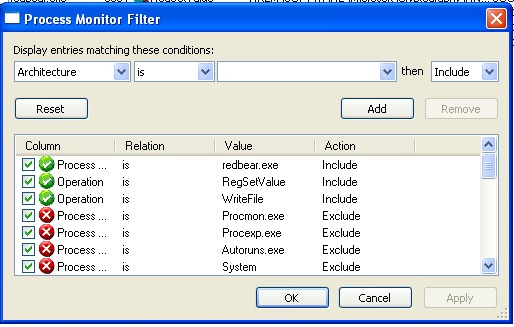
\includegraphics[width=0.4\linewidth]{fig6.jpeg}
            \caption{Filters applied}
            \label{6}
        \end{figure}
        \newpage
        now, with filters, processes window looks like this :
        \\
        \begin{figure}[h!]
            \centering
            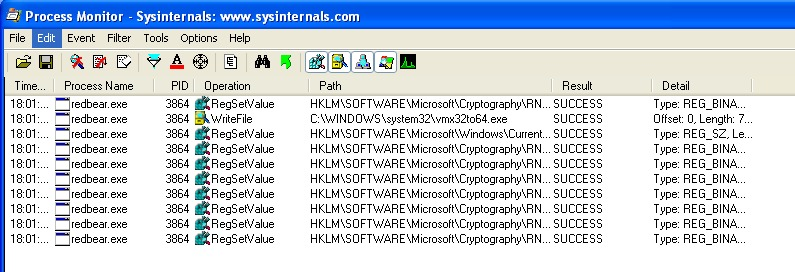
\includegraphics[width=0.4\linewidth]{fig7.jpeg}
            \caption{Processes filtered}
            \label{7}
        \end{figure}
        looking at the specific processes in process monitor, we can see that
        redbear created a key called videodriver . this key initialize the proccess of.

        \\ Now, we can apreciate that the size of redbear is $ 7kB  $  , also,
        the space of the file that was created is also $ 7kB  $ , that is
        supicious because it can mean that the file is exactly the same:
        \\
        \begin {figure} [h]
        \centering
        \begin {tabular}{c c}
        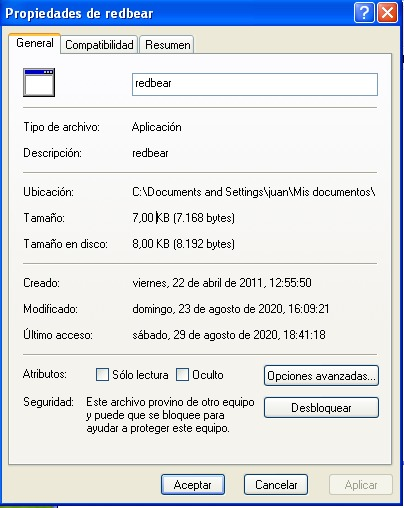
\includegraphics[width=0.3\linewidth]{img1.jpeg}
        &
        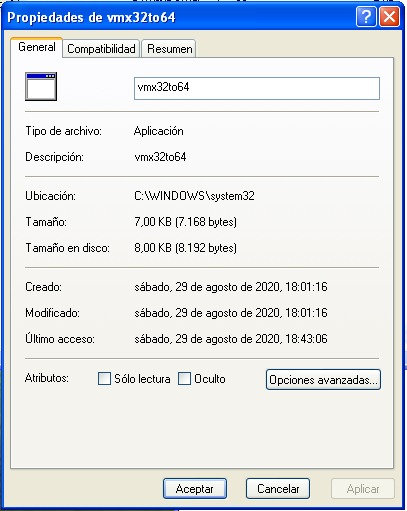
\includegraphics[width=0.3\linewidth]{img2.jpeg}
        \end {tabular}
        \caption{Sizes of both executables}
        \end {figure}
        \\
        for checking is the file is the same, we are going to check de
        hash,there are many hashing algorithm but we are going to use MD5.

        \\
        \begin{figure}[h]
            \centering
            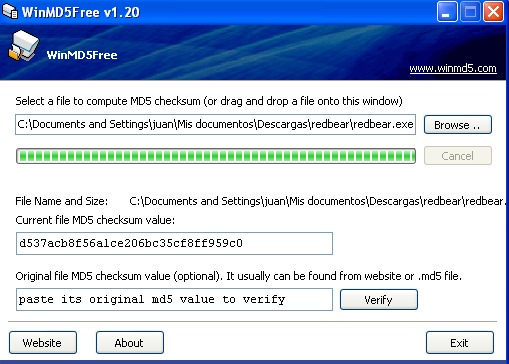
\includegraphics[width=0.4\linewidth]{hash1.jpeg}
            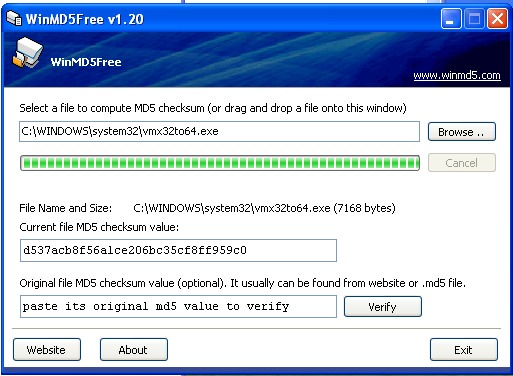
\includegraphics[width=0.4\linewidth]{hash2.jpeg}
            \\
            \caption{Hashes MD5 of both files}
            \label{hashes}
        \end{figure}

        \\ As we can see they are the same file !  :O , it means the program
        cloned itself to another path to hide from the owner of the machine.
            \begin{figure}[h!]
                \centering
                \color{blue}
                this was our reaction when we saw that the hashes were the same : ¿Its  a Colission?
                \color{black}
                \incfig{reaction}
                \caption{reaction}
                \label{fig:reaction}
            \end{figure}
        \newpage
        \section{Process explorer}
            We proceed to exectute process explorer :
            \begin{figure}[h!]
                \centering
                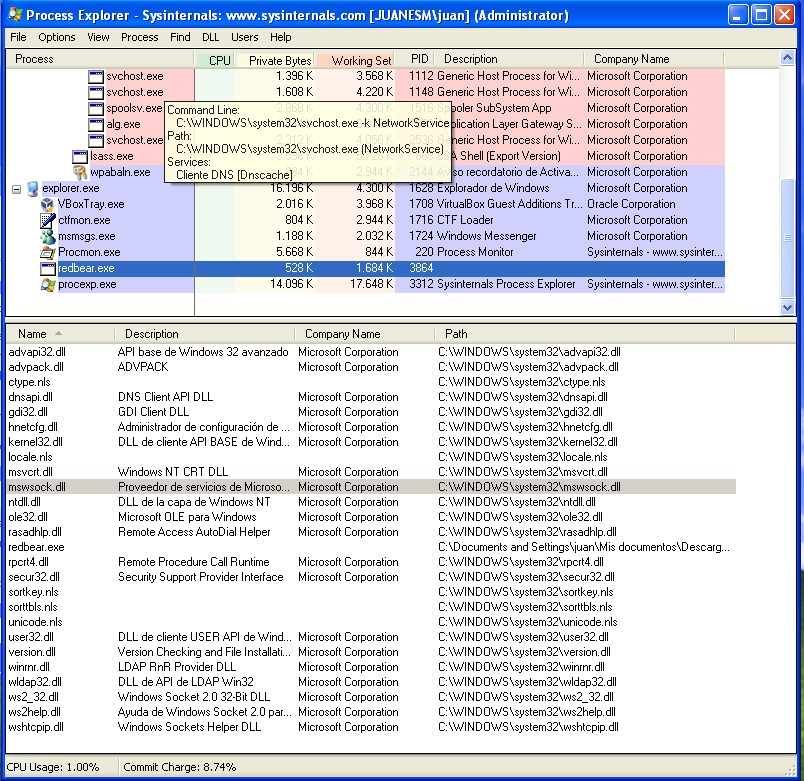
\includegraphics[width=0.6\linewidth]{fig9.jpeg}
                \caption{Process explorer execution}
                \label{9}
            \end{figure}
            in the lower part of the window we can apreciate the .dlls that the process is using.
            \\ among them we can find libraries like :
            \begin{itemize}
                \item {advapi32}
                \item {kernel32}
                \item {user32}
                \item {secure32}
            \end{itemize}
            now proceed to check the metadata of the file : this can be
            interesting because we can see information about the file, such as
            the date when it was created and the type of binary it is.
            \\
            \begin{figure}[h!]
                \centering
                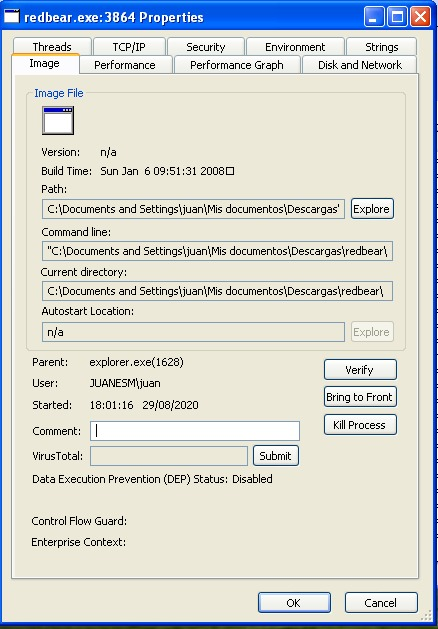
\includegraphics[width=0.4\linewidth]{fig10.jpeg} \\
                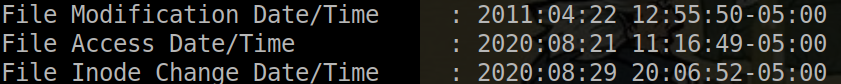
\includegraphics[width=0.4\linewidth]{meta.png}
                \caption{Metadata}
                \label{10}
            \end{figure}
            the "verify" button works when you want to check that the
            signatures inside the file are valid.

            \newpage
            \\ The strings in disk are the same that the strings in execution :
            \\
            \begin{figure}[h!]
                \centering
                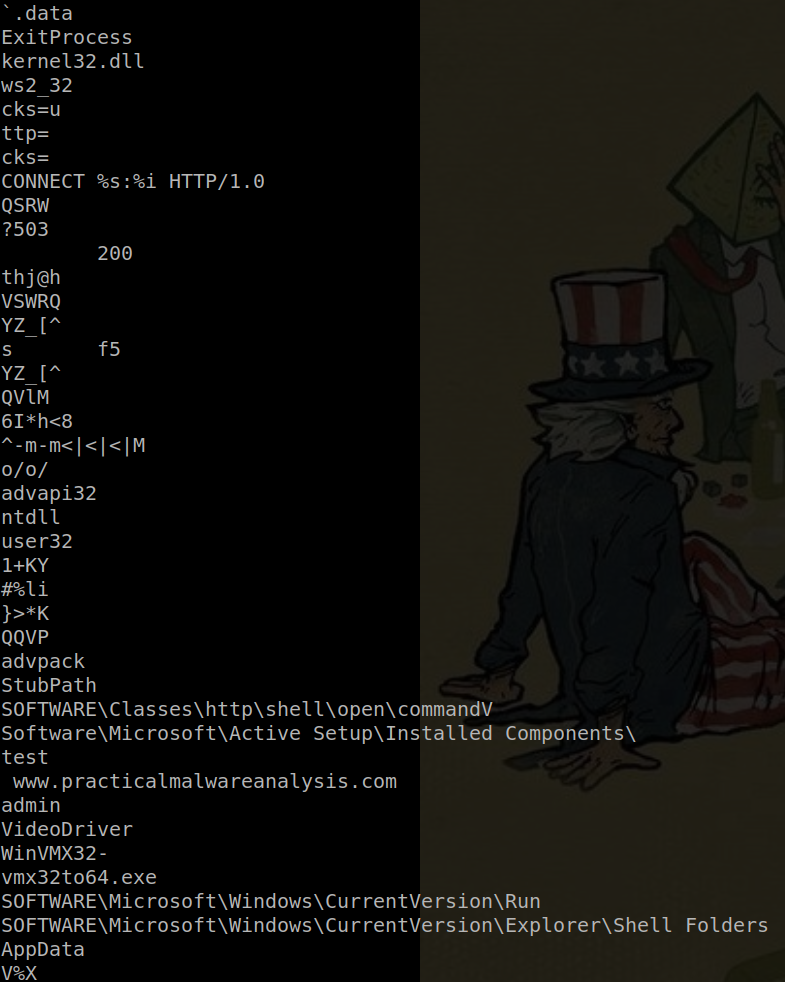
\includegraphics[width=0.4\linewidth]{strings1.png}
                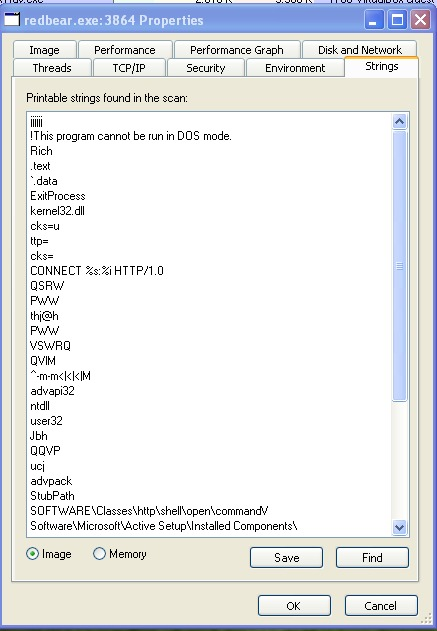
\includegraphics[width=0.4\linewidth]{strings2.jpeg}
                \caption{Strings}
                \label{11}
            \end{figure}

            \\ handles:
            \begin{figure}[h!]
                \centering
                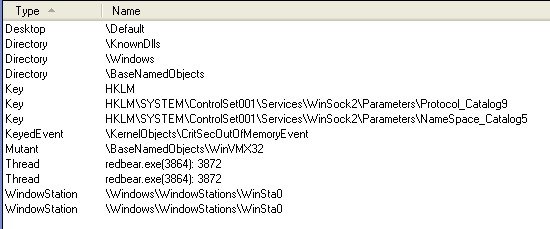
\includegraphics[width=0.5\linewidth]{handles.jpeg}
                \caption{Handles}
                \label{fig:handles}
            \end{figure}

            \\
            Mutant referst that is a modification of the original malware ,
            with different hash.
            \subsection{\color{red} ws2\_32.dll and wshtcpip.dll \color{black}  libraries}
                library ws2\_32.dll works for networking processes, but it also
                works for exhausting processes,processes that overcharge
                processors and make the machine slower.
                \\ wshtcpip library works for networking processes , is the
                library that handle tcp connections, as we know that redbear is
                a trojan, this library is the one that is going to send the
                conection to an attacker-host machine.
                \begin{figure}[h!]
                    \centering
                    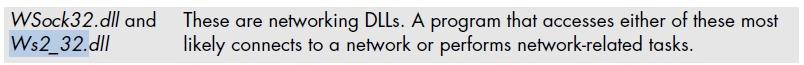
\includegraphics[width=0.9\linewidth]{libs.jpeg}
                    \caption{Libs}
                    \label{fig:libs}
                \end{figure}






















    %======================NOTES ENDS HERE===================%

    % bib stuff
    \nocite{*}
    \addtocontents{toc}{\protect\vspace{\beforebibskip}}
    \addcontentsline{toc}{section}{\refname}
    \bibliographystyle{plain}
    \bibliography{../Bibliography}
\end{document}
